%!TEX root = ../DissertationDefensePresentation.tex

{
\usebackgroundtemplate{
  
\begin{tikzpicture}
    \path [outer color = white, inner color = gray!85]
      (0,0) rectangle (\paperwidth,\paperheight);
  \end{tikzpicture}}
\begin{frame}
    \begin{textblock}{1.0}(0.00,0.20)
        \begin{tcbraster}[raster columns=2,raster force size=false,size=fbox]
            \begin{center}
                \tcbincludegraphics[blank,arc=\ClipSep,hbox,graphics options={width=0.4\textwidth}]{\figpath/1280px-CERN-aerial_1.jpg}\hspace*{0.1cm}\tcbincludegraphics[blank,arc=\ClipSep,hbox,graphics options={width=0.4\textwidth}]{\figpath/CMS_detector-s.jpg}
            \end{center} 
        \end{tcbraster}
    \end{textblock}
    \begin{textblock}{1.0}(0.0,0.75)
        \begin{center}
            \Huge
            Experimental Facilities\\
            \large
            CERN, the LHC, and CMS
        \end{center}
    \end{textblock}
\end{frame}
}

%%--------------------------------------------------------------------------------------------

\subsection*{CERN}

%%--------------------------------------------------------------------------------------------

\begin{frame}
    \frametitle{CERN}
    \framesubtitle{European Organization for Nuclear Research}
    \vspace*{-0.44cm}
    \begin{columns}[T]
        \begin{column}{0.4\textwidth}
            \begin{block}{}
                \begin{itemize}
                    \item One of the world's premier particle physics laboratories
                    \begin{itemize}
                        \item Founded in 1954
                        \item Currently supported by 22 member states
                        \item Located along the French-Swiss border near Geneva, Switzerland
                        \item Many discoveries: \PW, \PZ, and \PH bosons, World Wide Web, etc.
                    \end{itemize}
                    \vspace*{0.2cm}
                    \item A huge underground accelerator complex supports the largest of the beamlines, the Large Hadron Collider (LHC)
                \end{itemize}
            \end{block}
        \end{column}
        \begin{column}{0.58\textwidth}
            \centering
            \vspace*{1.0cm}
            \hspace*{0.1cm}\includegraphics[width=\figwidth]{\figpath/CERN-LHC.jpg}
        \end{column}
    \end{columns}
\end{frame}

%%--------------------------------------------------------------------------------------------

\subsection*{Large Hadron Collider (LHC)}

%%--------------------------------------------------------------------------------------------

\frame{
    \frametitle{The Large Hadron Collider (LHC)}
    \vspace*{-0.24cm}
    \begin{columns}[T]
        \column{0.58\textwidth}
            \vspace*{0.6cm}
            \begin{block}{}
                \begin{itemize}
                    \item Proton-proton collider
                    \begin{itemize}
                        \item 27\unit{km} circumference
                        \item $\sim$100\unit{m} underground
                        \item Design center of mass energy of 14\TeV
                        \item Crossing rate 25\unit{ns}
                    \end{itemize}
                    \vspace*{0.2cm}
                    \item This analysis uses the full 2012 dataset
                    \begin{itemize}
                        \item \CM{8\tev}, 50\unit{ns}
                        \item $\int \mathcal{L}\sim$19.148 (19.279)\fbinv for electrons (muons)
                    \end{itemize}
                    \vspace*{0.2cm}
                    \item Two general purpose detectors (\textbf{CMS} \& ATLAS) and several other specialized experiments
                \end{itemize}
            \end{block}
        \column{0.4\textwidth}
            \hspace*{0.1cm}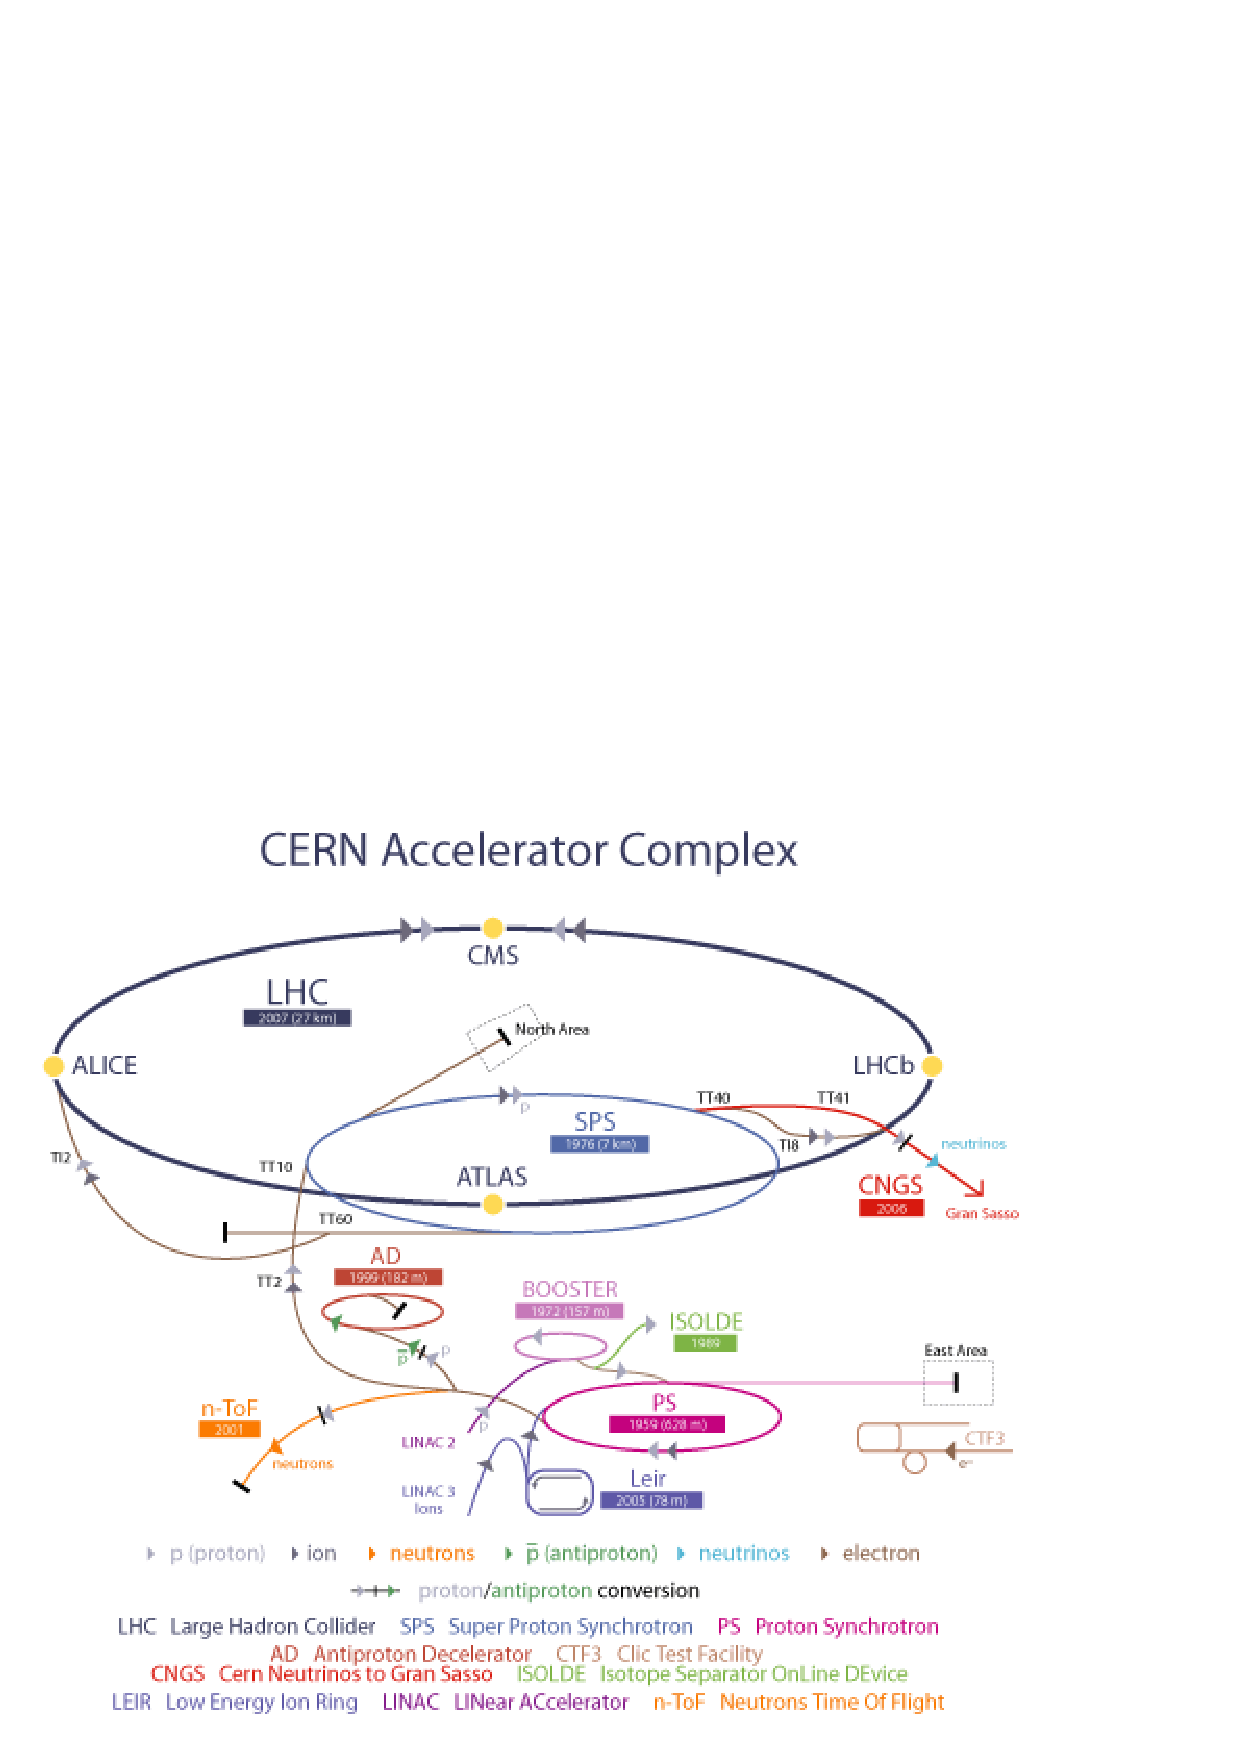
\includegraphics[width=\figwidth]{\figpath/AccComplex.pdf}\\
            \hspace*{0.1cm}\includegraphics[width=\figwidth]{\figpath/int_lumi_cumulative_pp_2.pdf}
    \end{columns}
}

%%--------------------------------------------------------------------------------------------

\subsection*{Compact Muon Solenoid (CMS)}

%%--------------------------------------------------------------------------------------------

\frame{
    \frametitle{The Compact Muon Solenoid (CMS)}
    \vspace*{-0.24cm}
    \begin{block}{}
        \begin{itemize}
            \small
            \item Standard multipurpose detector, benefits from:
            \begin{itemize}
                \footnotesize
                \item High magnetic field
                \item High granularity tracker (lepton finding)
                \item Excellent electromagnetic calorimeter resolution
                \item Good particle identification due to the particle flow (PF) algorithm
            \end{itemize}            
        \end{itemize}
    \end{block}
    \begin{columns}[T]
        \begin{column}{0.65\textwidth}
            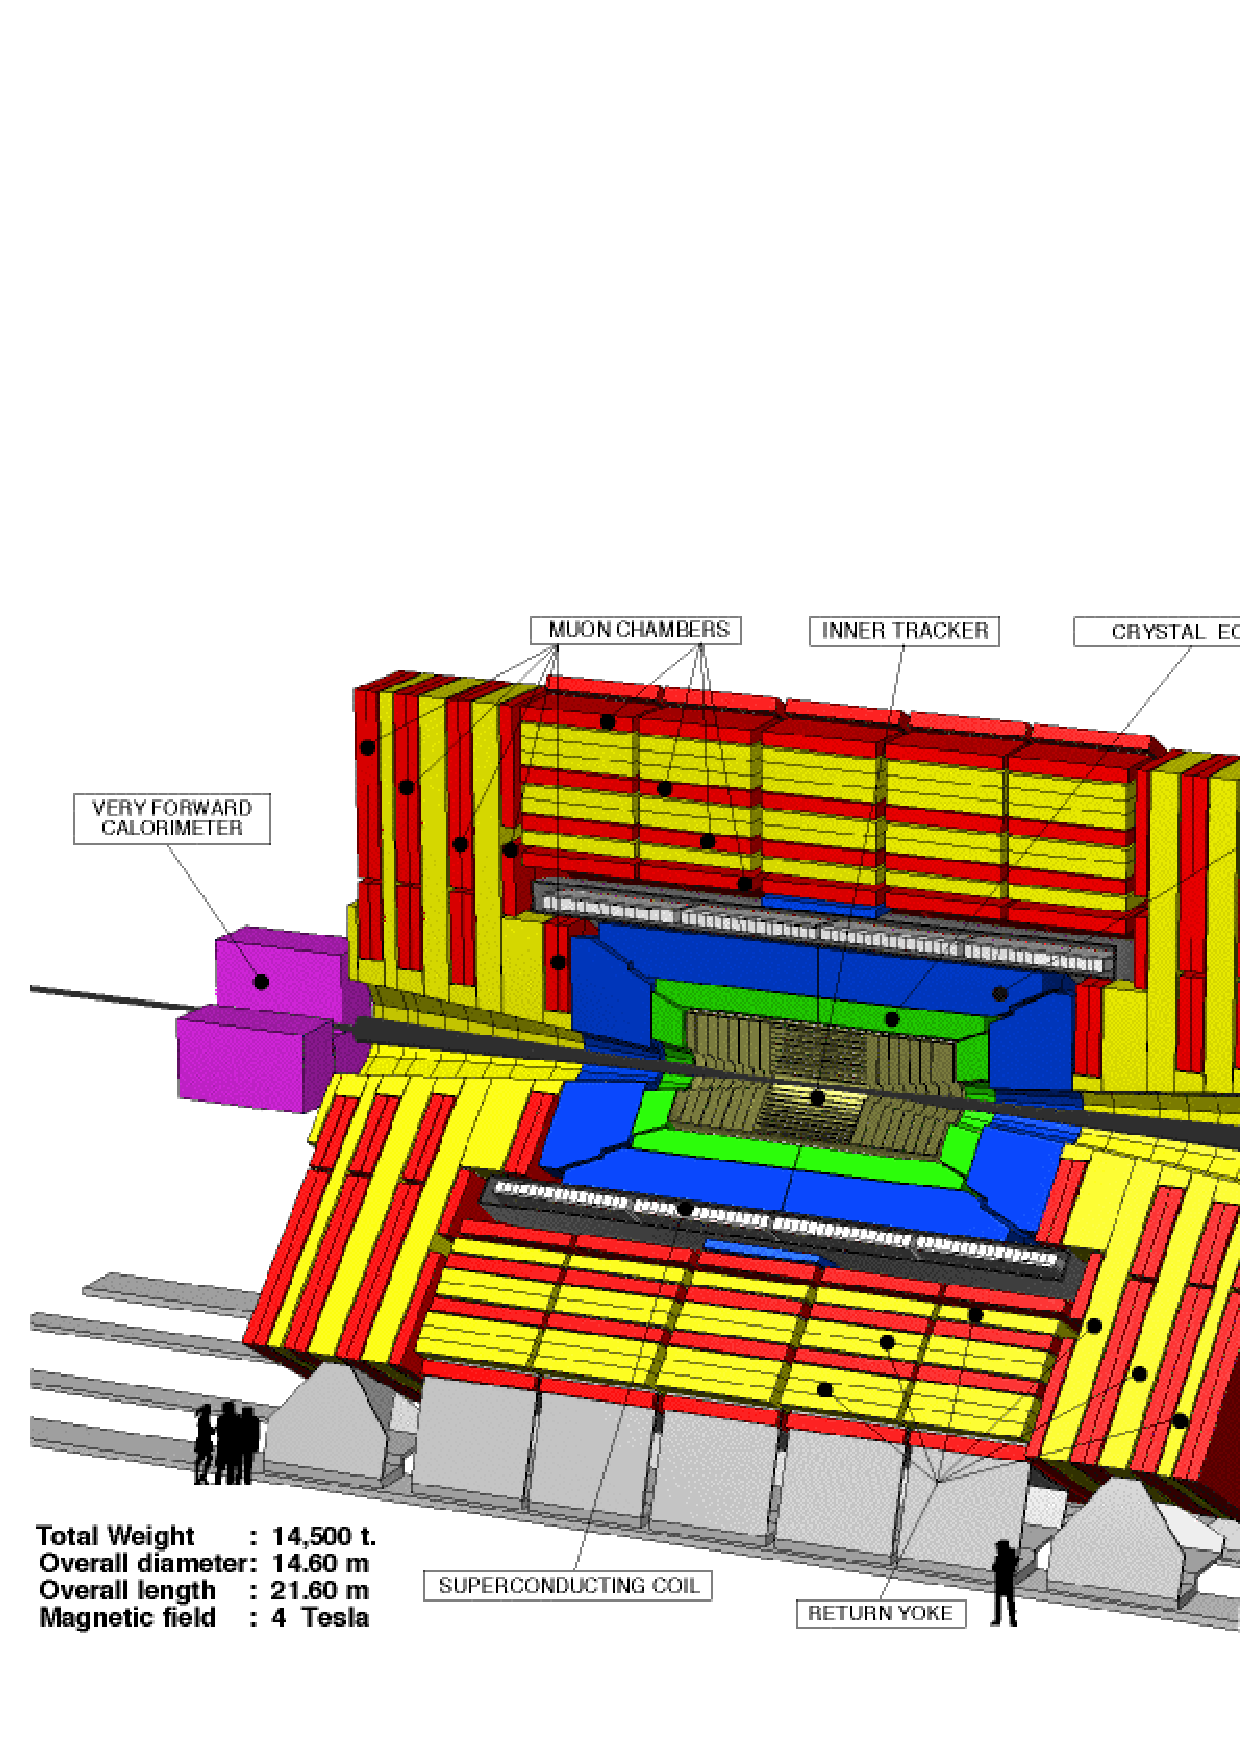
\includegraphics[width=\textwidth]{\figpath/cms.png}
        \end{column}
        \begin{column}{0.35\textwidth}
            \begin{figure}
                \centering
                \includegraphics[width=\textwidth]{\figpath/dimuon_logo.png}
            \end{figure}
            \vfill
            \begin{figure}
                \centering
                \includegraphics[width=\textwidth]{\figpath/diphoton_v2.png}
            \end{figure}
        \end{column}
    \end{columns}
}

\begin{frame}%<1>[label=frame:definitions]
    \setbeamercovered{transparent}
    \frametitle{Definitions}
    \vspace*{-0.24cm}
    \begin{block}{Coordinate System}
        \begin{columns}[T]
            \column{0.5\textwidth}
                \begin{itemize}
                    \scriptsize{
                      \item z-axis - Along the beam pipe
                      \item $\phi$ - The azimuthal angle
                      \item $\eta=-ln[tan(\frac{\theta}{2})]$ (called pseudorapidity)
                      \item $p_{T}$ - The transverse momentum (in the x-y plane)
                    }
                \end{itemize}
            \column{0.5\textwidth}
                \includegraphics[width=0.53\textwidth]{\figpath/gem_sketch.png}
                \includegraphics[width=0.45\textwidth]{\figpath/Pseudorapidity2.png}
        \end{columns}
    \end{block}
    \vspace*{-0.16cm}
    \begin{block}{Physics Objects}
        \begin{columns}[T]
            \column{0.45\textwidth}
                \begin{itemize}
                    \scriptsize{
                        \uncover<2->{\item Leptons {\color{gray}(Hadrons/Photons)}}
                        \uncover<3->{\item $\Em_{T}$ - Missing transverse energy
                        \begin{itemize}
                            \scriptsize{
                                \item Intrinsically from neutrinos
                                \item Indirectly from:
                                \begin{itemize}
                                    \scriptsize
                                    \item Jet Mismeasurements
                                    \item Detector Noise
                                    \item Pileup (multiple hard scatter interactions per bunch crossing)
                                \end{itemize}
                            }
                        \end{itemize}}
                        \uncover<4->{\item Jet - Collimated spray of particles
                        \begin{itemize}
                            \scriptsize{
                                \item Resulting from the hadronization of quarks and gluons
                            }
                        \end{itemize}}
                    }
                \end{itemize}
            \column{0.55\textwidth}
                \vspace*{-0.2cm}
                \begin{center}
                    \only<1-2>{\vspace*{0.25cm}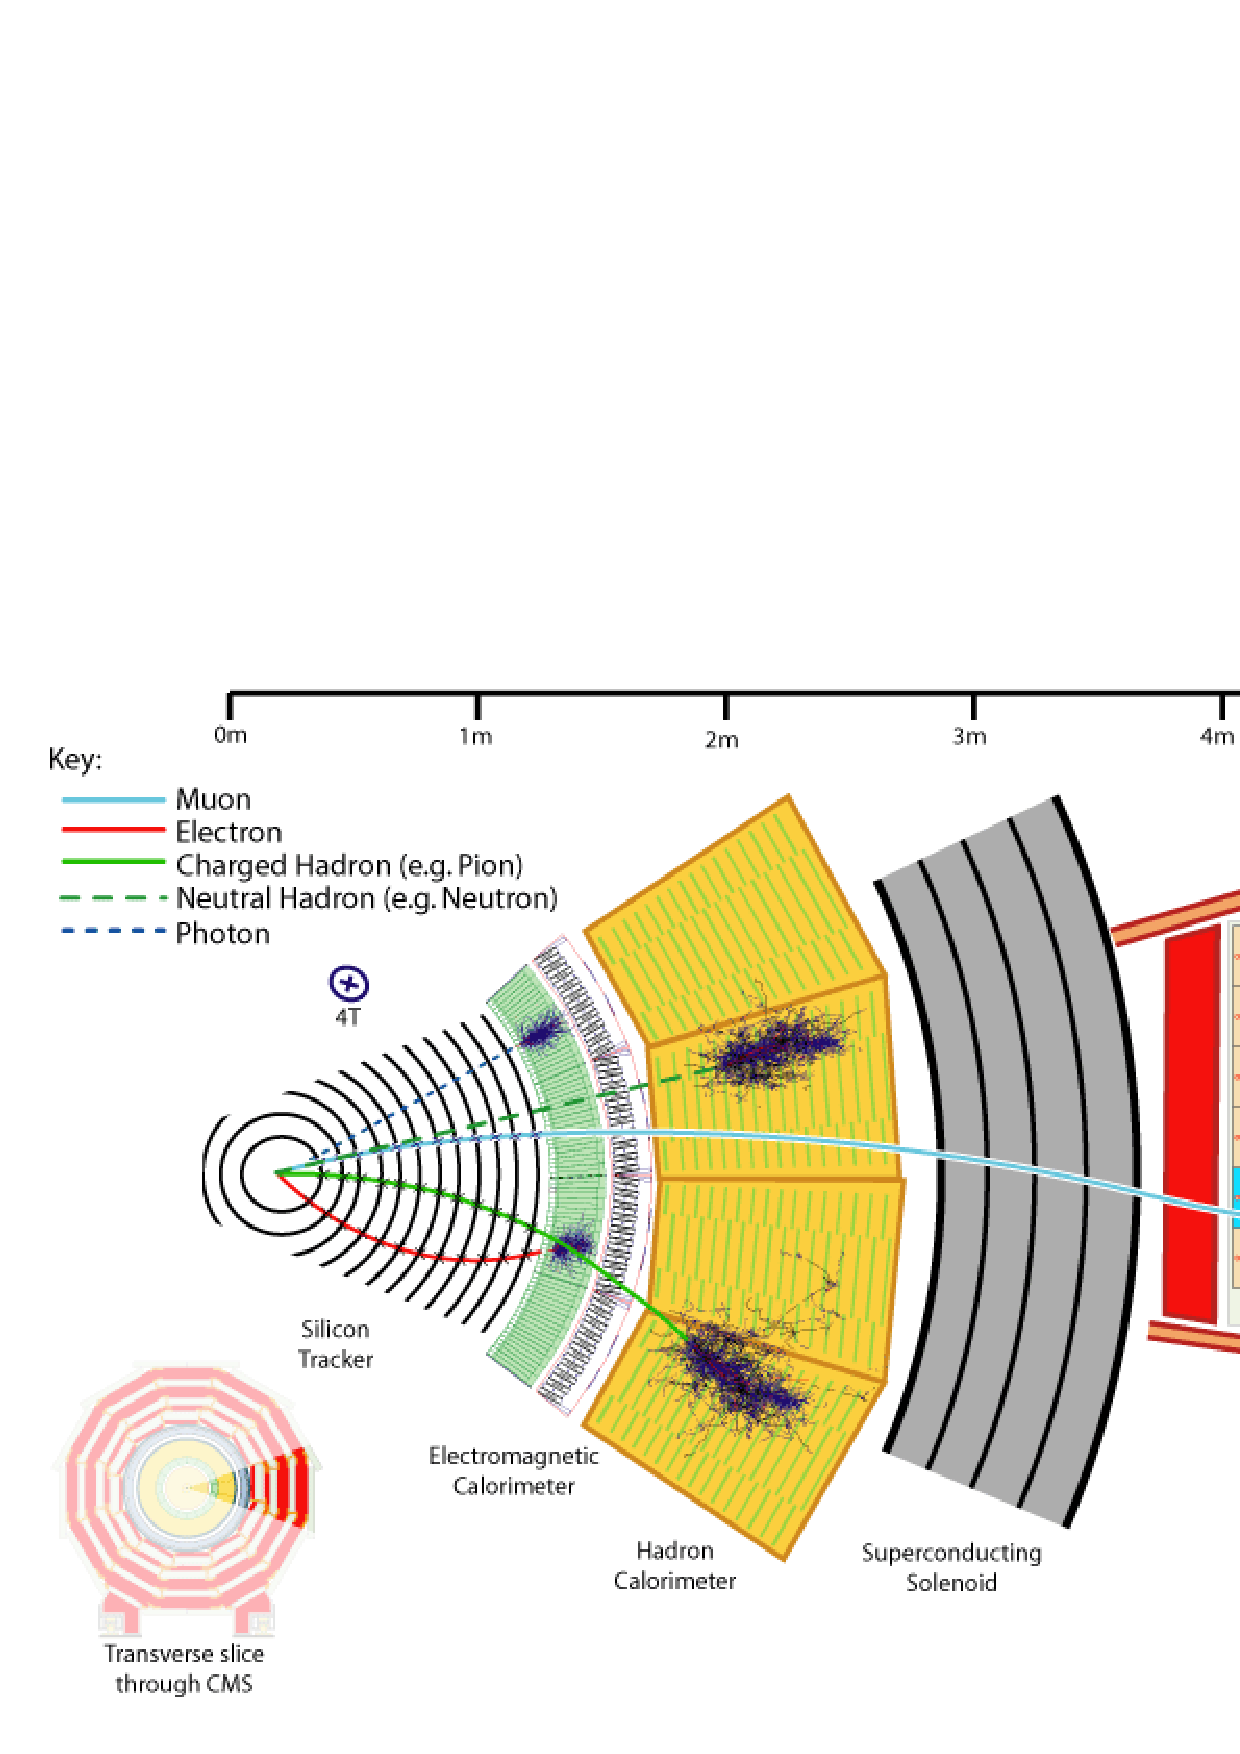
\includegraphics[width=\textwidth]{\figpath/CMS_Slice.pdf}}
                    %\only<3>{\includegraphics[width=0.8\textwidth]{\figpath/MEt.png}}
                    \only<3>{
                        \vspace*{-0.05cm}
                        \hspace*{0.95cm}\begin{tikzpicture}[scale=0.9]
                            \node[inner sep=0pt] {\includegraphics[width=0.65\textwidth]{\figpath/CMSWireframe_compressed.png}};
                            \draw[blue, thick, arrow] (0.0,0.0) -- (0.6,0.6) node[xshift=-0.8cm] {\footnotesize muon $p_{T}$};
                            \draw[blue, thick, arrow] (0.0,0.0) -- (1.4,-1.0) node[midway,left] {\footnotesize jet $p_{T}$};
                            \draw[orange, thick, arrow] (1.4,-1.0) -- (2.0,-0.4) node[midway,right, xshift=0.22cm, yshift=-0.1cm, text width=1.5cm] {\footnotesize shifted muon $p_{T}$};
                            \draw[Goldenrod, thick, arrow] (0.0,0.0) -- (2.0,-0.4) node[midway,xshift=0.25cm, yshift=0.25cm] {\footnotesize $\sum_{\text{\scriptsize objects}} p_{T}$};
                            \draw[green, thick, arrow] (0.0,0.0) -- (-2.0,0.4) node[xshift=0.5cm,yshift=0.25cm] {\footnotesize \VETslash};
                            \node[outer sep=1pt, text=Goldenrod] at (2.4,-1.8) {\tiny x};
                            \node[outer sep=1pt, text=Goldenrod] at (1.95,-1.35) {\tiny y};
                            \node[outer sep=1pt, text=Goldenrod] at (1.95,-1.8) {\tiny z};
                        \end{tikzpicture}
                    }
                    \only<4>{\includegraphics[width=0.4\textwidth]{\figpath/display_xy_annotated.png}}
                \end{center}
        \end{columns}
    \end{block}
\end{frame}
%\againframe<2>{frame:definitions}
%\againframe<3>{frame:definitions}
%\againframe<4>{frame:definitions}